\begin{figure}
	\centering
	\begin{subfigure}{0.45\textwidth}
		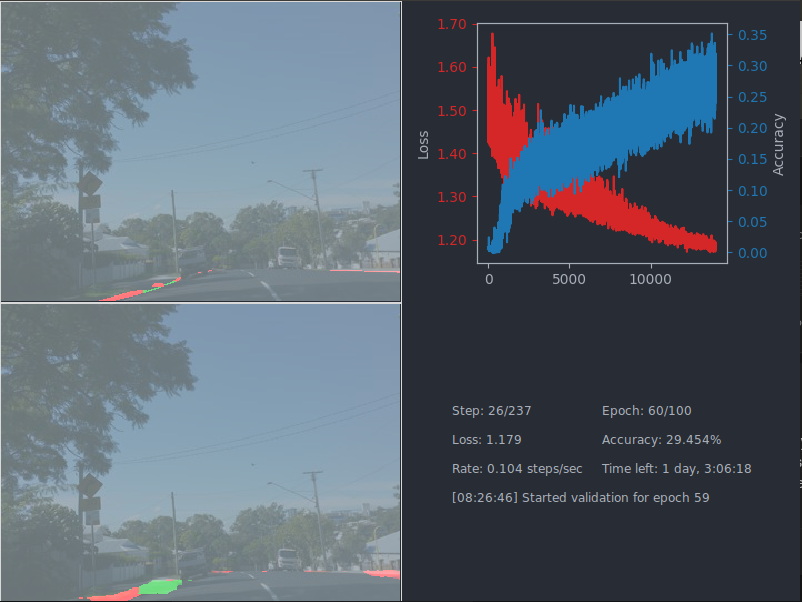
\includegraphics[width=\linewidth]{figures/experiments/gui.png}
		\caption[Training GUI]{A screen capture of the GUI that was used to visualize training results. In clockwise from the top left, the GUI visualizes the ground truth data, a live plot of the loss and accuracy, various statistics, and the network output.}
		\label{fig:experiments-gui}
	\end{subfigure}
	\hfill
	\begin{subfigure}{0.45\textwidth}
		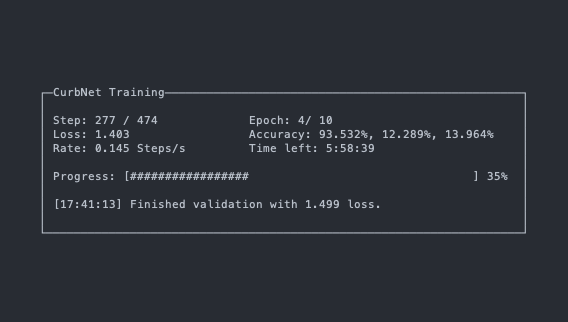
\includegraphics[width=\linewidth]{figures/experiments/cli.png}
		\caption[Training CLI]{A screen capture of the CLI that was used to train the network remotely.}
		\label{fig:experiments-cli}
	\end{subfigure}
	\caption[Training UI]{The two available user interfaces available to use with CurbNet. The GUI was mean to more simply and quickly deliver the most important information first to the researcher. The CLI was designed to allow training status along with the most pertinent information to be shown remotely with little overhead.}
\end{figure}